% We need layers to draw the block diagram
\pgfdeclarelayer{background}
\pgfdeclarelayer{foreground}
\pgfsetlayers{background,main,foreground}

% Define a few styles and constants
\tikzstyle{sensor}=[draw, fill=blue!20, text width=5em,text centered, minimum height=2.5em]
\tikzstyle{system} = [sensor, text width=6em, fill=green!30, 
    minimum height=12em, rounded corners]
\tikzstyle{input} = [coordinate]
\tikzstyle{sum} = [draw, fill=blue!20, circle, node distance=1cm]
%\tikzstyle{output} = [coordinate]
\def\blockdist{0.5}
\def\edgedist{0.7}
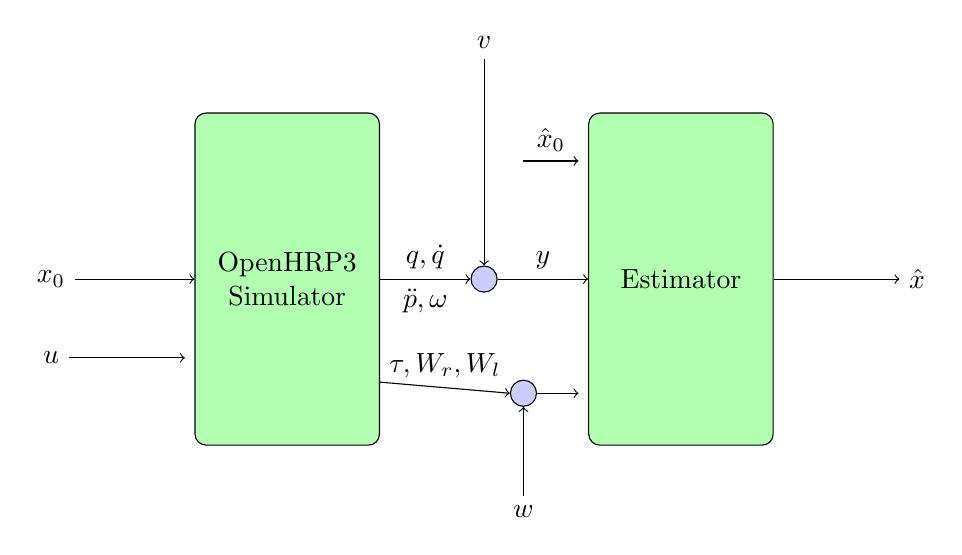
\begin{tikzpicture}
	% Define the nodes in the picture
	\node (sys_in)[yshift=1cm]{$x_0$};
	\node (u_in) [below of=sys_in,node distance=1cm]{$u$};
    \node (sim_sys) [system,right of=sys_in,node distance=3cm] {OpenHRP3 Simulator};
    \node (msr_add)[sum,right of=sim_sys,node distance=2.5cm]{};
    \node (msr_noise)[above of=msr_add,node distance=3cm]{$v$};
    \node (estimator) [system,right of=msr_add,node distance =2.5cm]{ Estimator};
    \node (est_in) [input,right of=sim_sys,node distance=3cm,yshift=1.5cm]{};
	\node (inp_add)[sum,right of=sim_sys, node distance=3cm,yshift=-1.45cm]{};    
	\node (sys_noise)[below of=inp_add,node distance=1.5cm]{$w$};
    \node (est_out)[right of=estimator,node distance=3cm]{$\hat{x}$};
    
    % Define the edges in the picture
    \draw [->] (sys_in) --node{}(sim_sys.west);
    \draw [->] (u_in) --node{}+(1.7,0);
	\draw [->] (sim_sys.-48.75) --node[above]{$\tau,W_r,W_l$}(inp_add.west);
    \draw [->] (inp_add) --node{}+(\edgedist,0);
	\draw [->] (sys_noise) --node{}(inp_add);
    \draw [->] (est_in) --node[above]{$\hat{x}_0$}+(\edgedist,0);

    \draw [->] (msr_noise) --node{}(msr_add.north);
    \draw [->] (sim_sys.east) --node[above]{$q,\dot{q}$}node[below]{$\ddot{p},\omega$}(msr_add.west);
    \draw [->] (msr_add.east) --node[above]{$y$}(estimator.west);
    \draw [->] (estimator) --node{}(est_out);
\end{tikzpicture}